\chapter{Proposed Solution}
Ideas:
\begin{itemize}
    \item Progress
        \begin{itemize}
            \item begin flat multilayer rendering
        \end{itemize}
\end{itemize}

We got inspired by a circular form of a tree map plot for hierarchical structures (see Figure \ref{fig:hierarchicalCirclePlot}). Each node can either be a simple leaf node or a network itself. So we need a way to visualize connections between different networks, a way to do this is a multilayer network visualization see Figure \ref{fig:2dmultilayerVis}. Here each flat layer represents a different network but a hierarchical relationship is not always given for these visualizations.  

\begin{figure}[h]
    \centering
    \begin{subfigure}[b]{0.40\columnwidth}
        \centering
        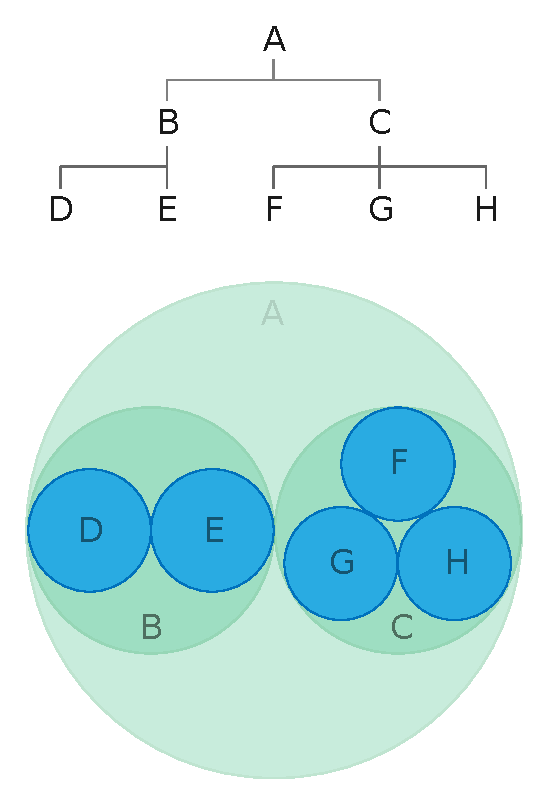
\includegraphics[width=\textwidth, trim={0 0 0 4.3cm},clip]{graphics/circle_packing.pdf}
        \subcaption{Hierarchical circle packing plot \cite{ribecca_circle_nodate}}
        \label{fig:hierarchicalCirclePlot}
    \end{subfigure}
    \begin{subfigure}[b]{0.50\columnwidth}
      \centering
      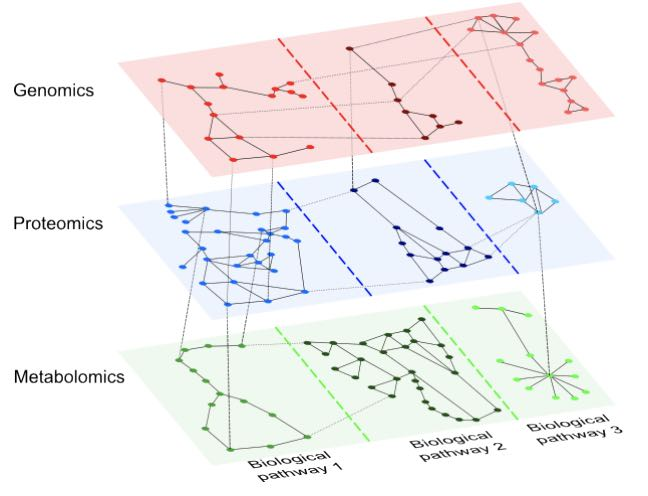
\includegraphics[width=\textwidth]{graphics/2dmultilayerVis.jpg}
      \subcaption{multilayer network visualization \cite{ghoniem_state_2019}}
      \label{fig:2dmultilayerVis}
    \end{subfigure}
    \caption[Optional caption for the figure list (often used to abbreviate long captions)]{Reference visualizations that we used as a starting point. (a) shows a possible visualization for hierarchical structures, (b) shows a visualization for networks with multiple layers} % Remove the [...] argument if the original caption should be used in the figure list.
    \label{fig:referenceVisualizations} 
  \end{figure}

\section{Concepts}
\subsection{Original 2D Visualization}
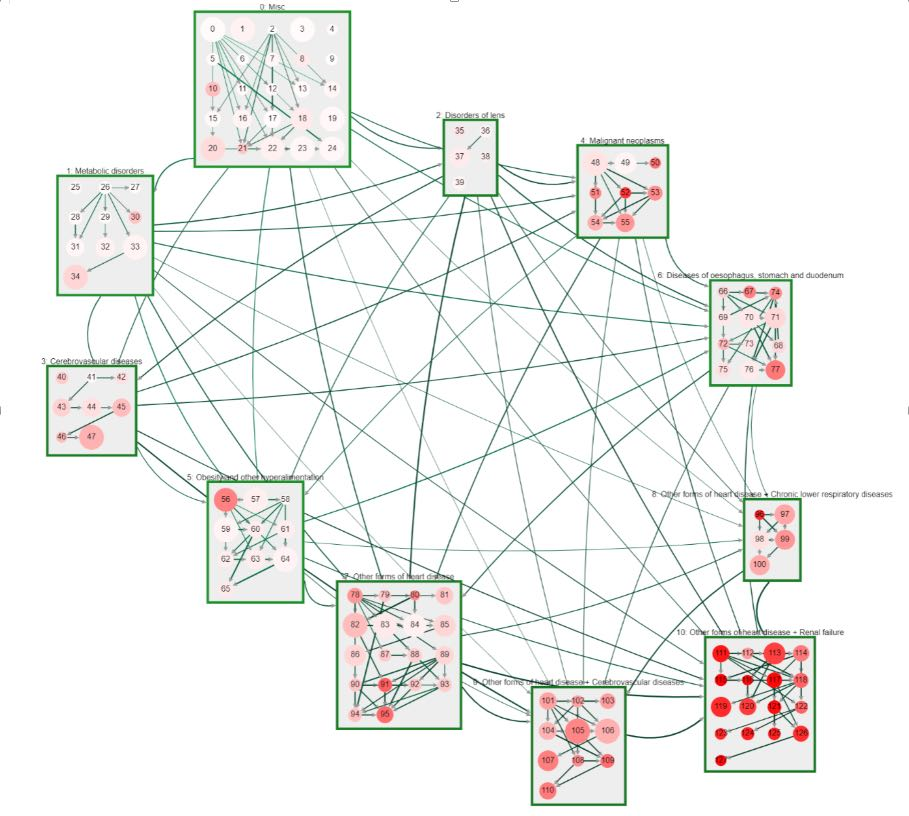
\includegraphics[width=0.5\textwidth]{chapters/graphics/2dVisOfDemoData.jpg}

Problem only two layers supported

\subsection{2-Layer Concept}
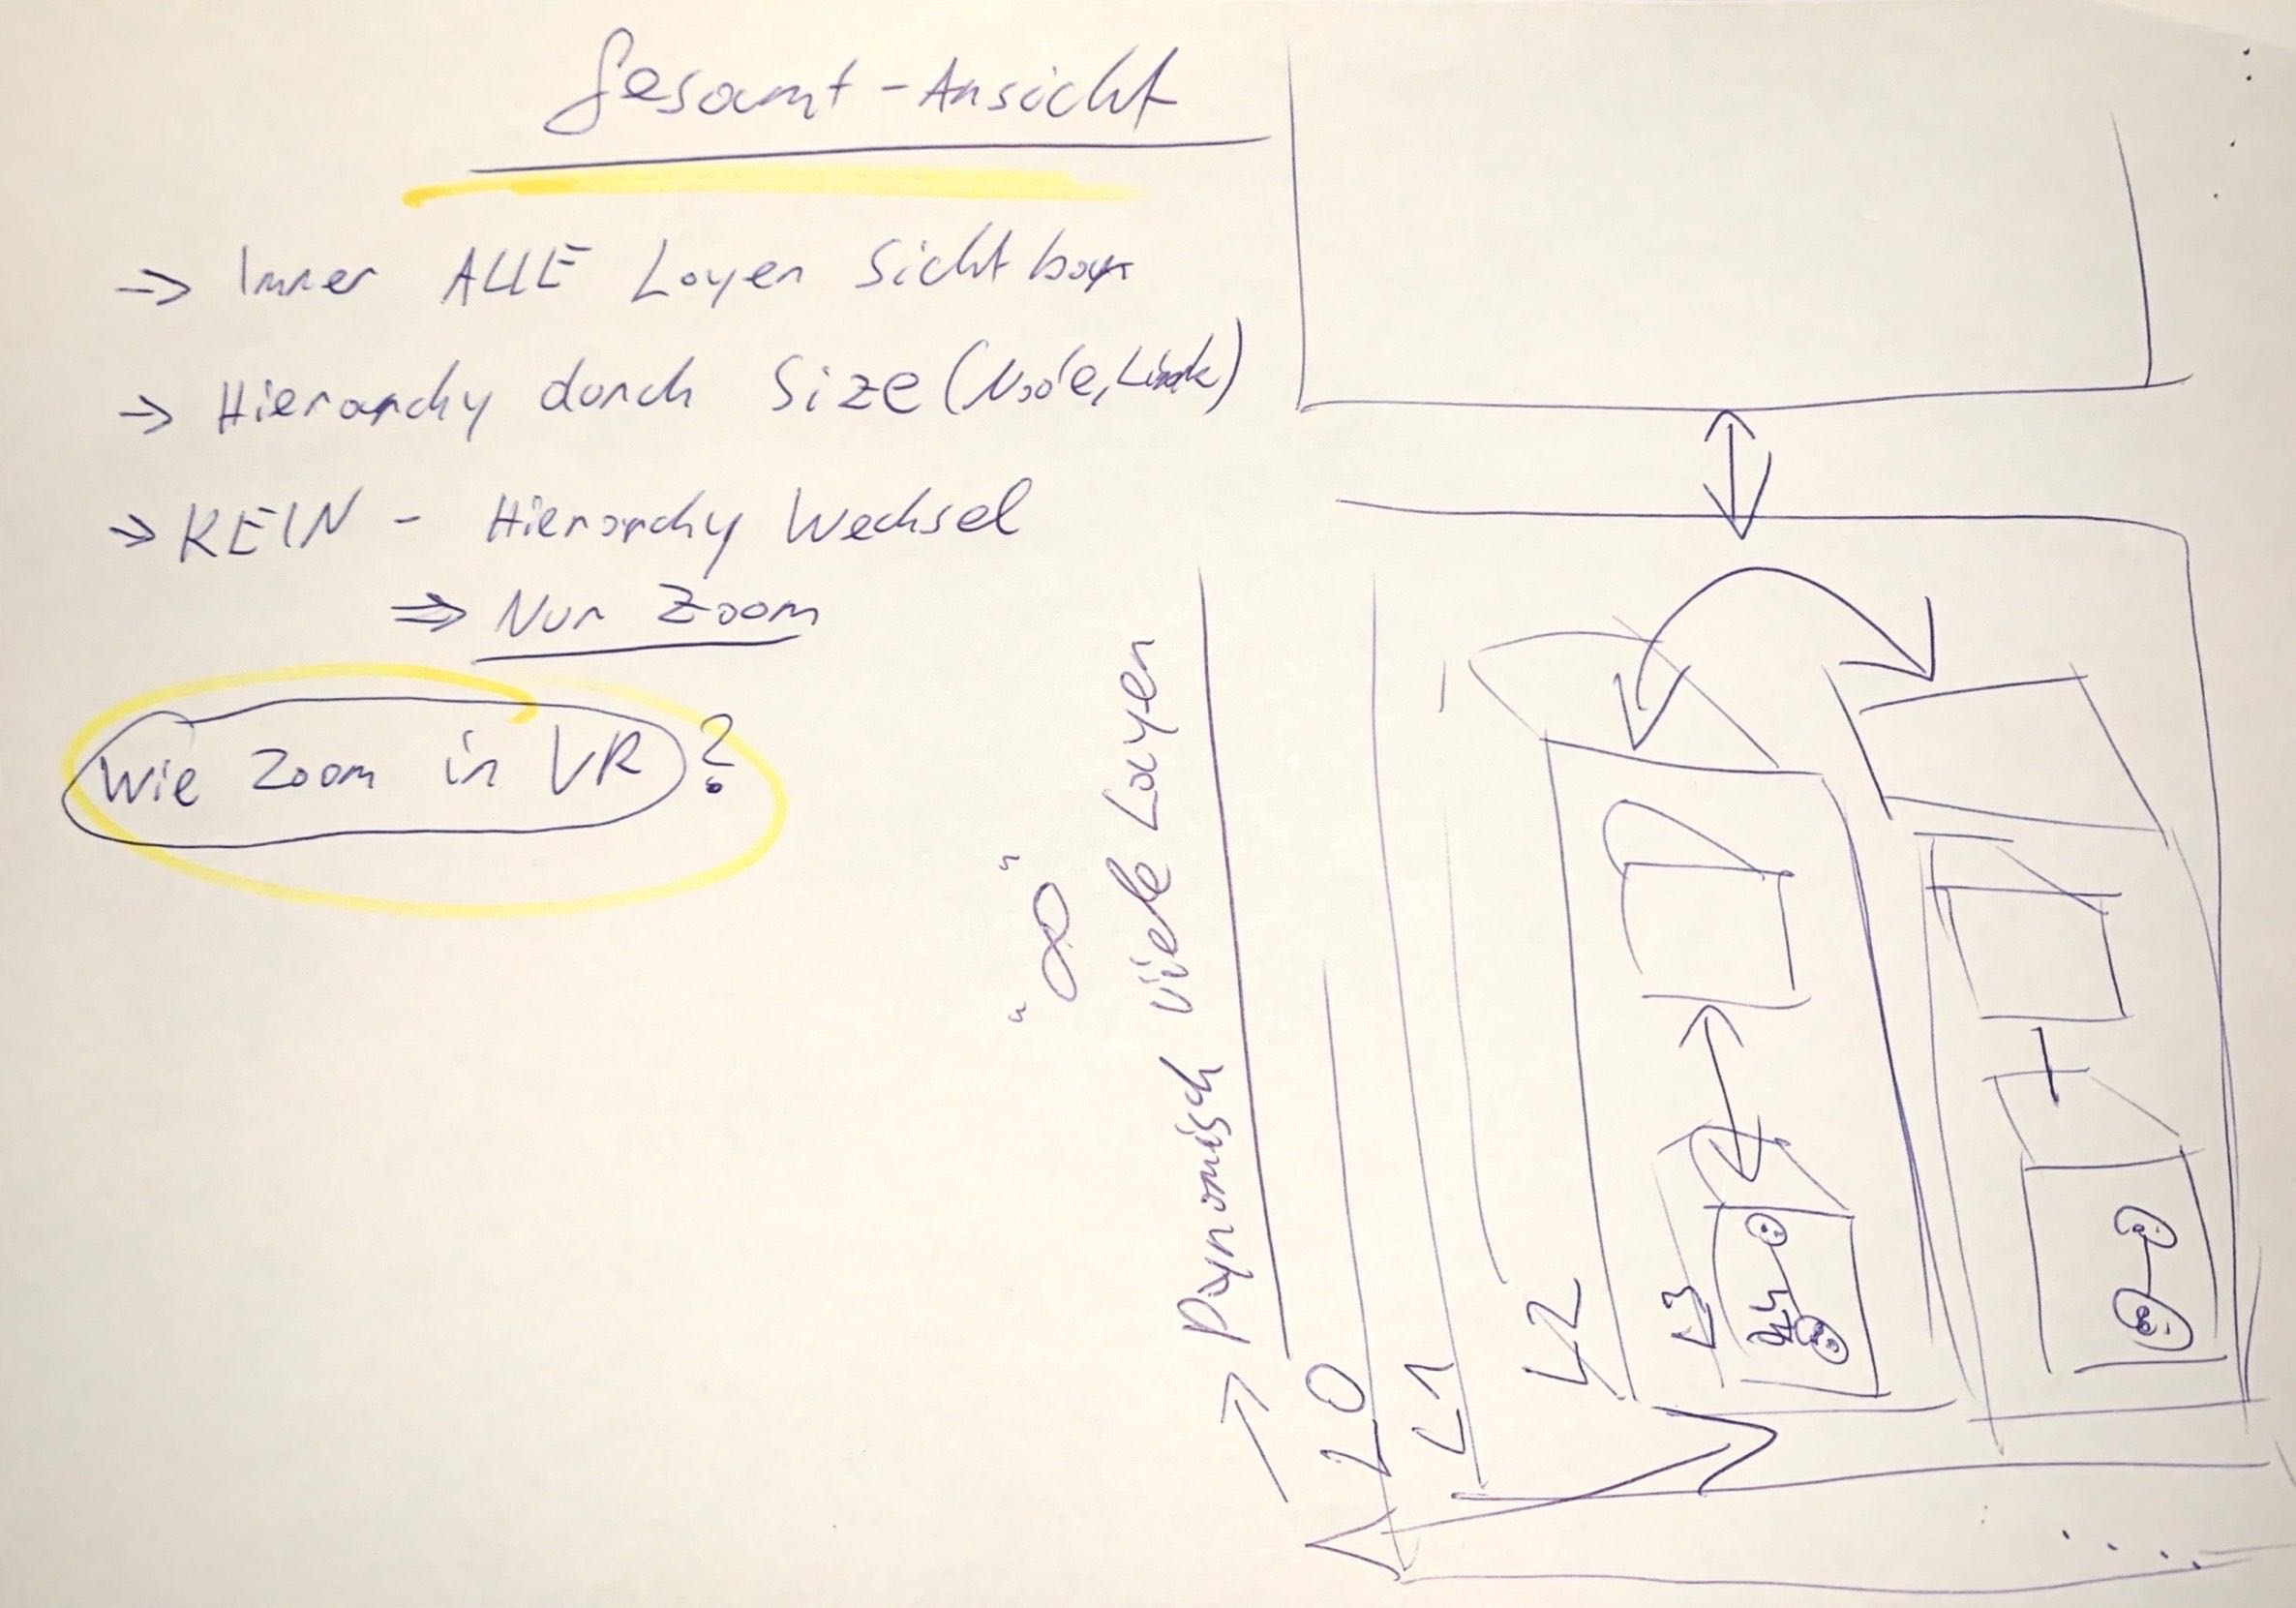
\includegraphics[width=0.5\textwidth]{chapters/graphics/concept2.jpg}

Cube/ (half) sphere position of sub-graphs \\
Starting idea, why it was discarded

\subsection{n-Layer Concept}
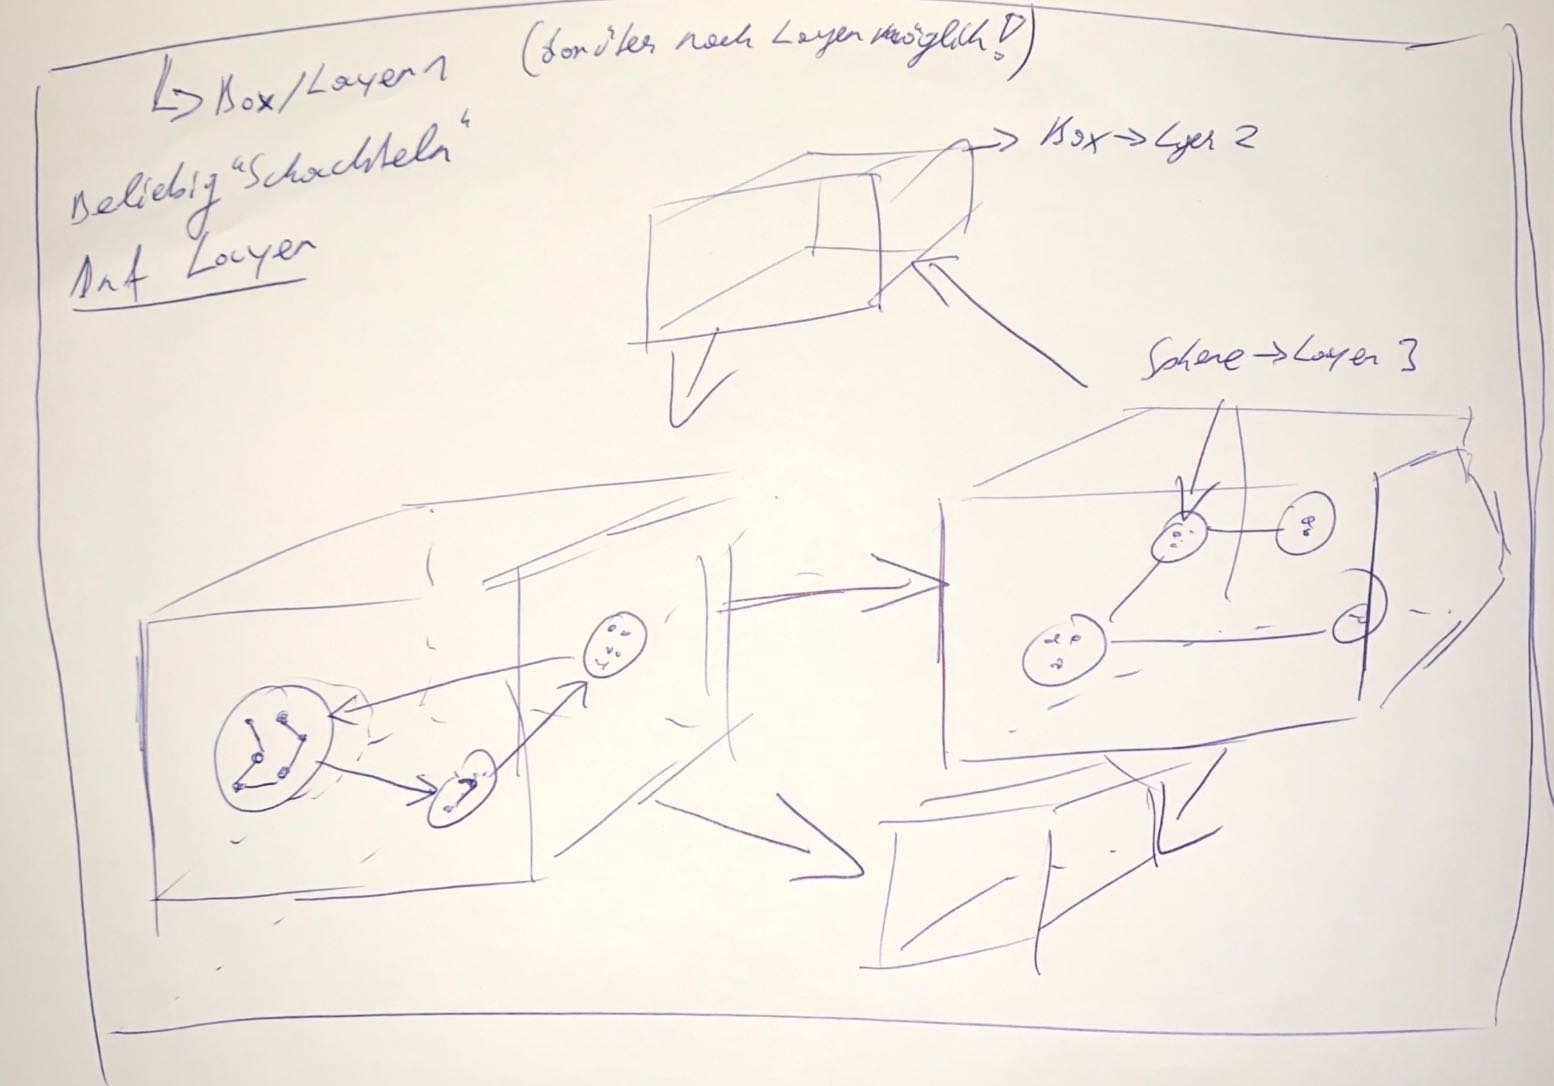
\includegraphics[width=0.5\textwidth]{chapters/graphics/concept1.jpg}

Improved concept \\
no fixed cube/(half) sphere position instead each layer calculate its own position \\
circle over boxes \\
Begin: flyspeed only, later on problem on VR \\

\section{Position of Nodes}

Independent per layer / sub-graph inside parent node \\
use of existing implemented and already good tested(prevents overlapping, good distribution, ...) forces (collision, link, manyBody, ...) \\
use of own forces to place sub-graphs inside parent graphs \\
adjustable force strengths \\
Node size grow with number of child nodes \\
\\
two possible solutions: web-worker vs live \\

\section{Usage of different Visual Features}

Position \\
linkWidth \\
linkColor \\
linkDirection \\ 
currentLayer on Controller Overlay \\ 

\section{Graph Exploration}

\subsection{Overview Layout}
Orbital Camera

\subsection{Detail Layout}
Free Fly Camera \\
change FlySpeed based on current node the camera is located. As deeper the layer as slower the flyspeed \\
Problem experiments showed this does not work well in VR --> manual / automated scaling. \\

flyToNode \\
flyToParentLayer \\

\subsection{Visibility of the Visualization}
\subsubsection{Nodes / Layers}
wireframe
\subsubsection{Links}
lockLinks

\section{Interaction}
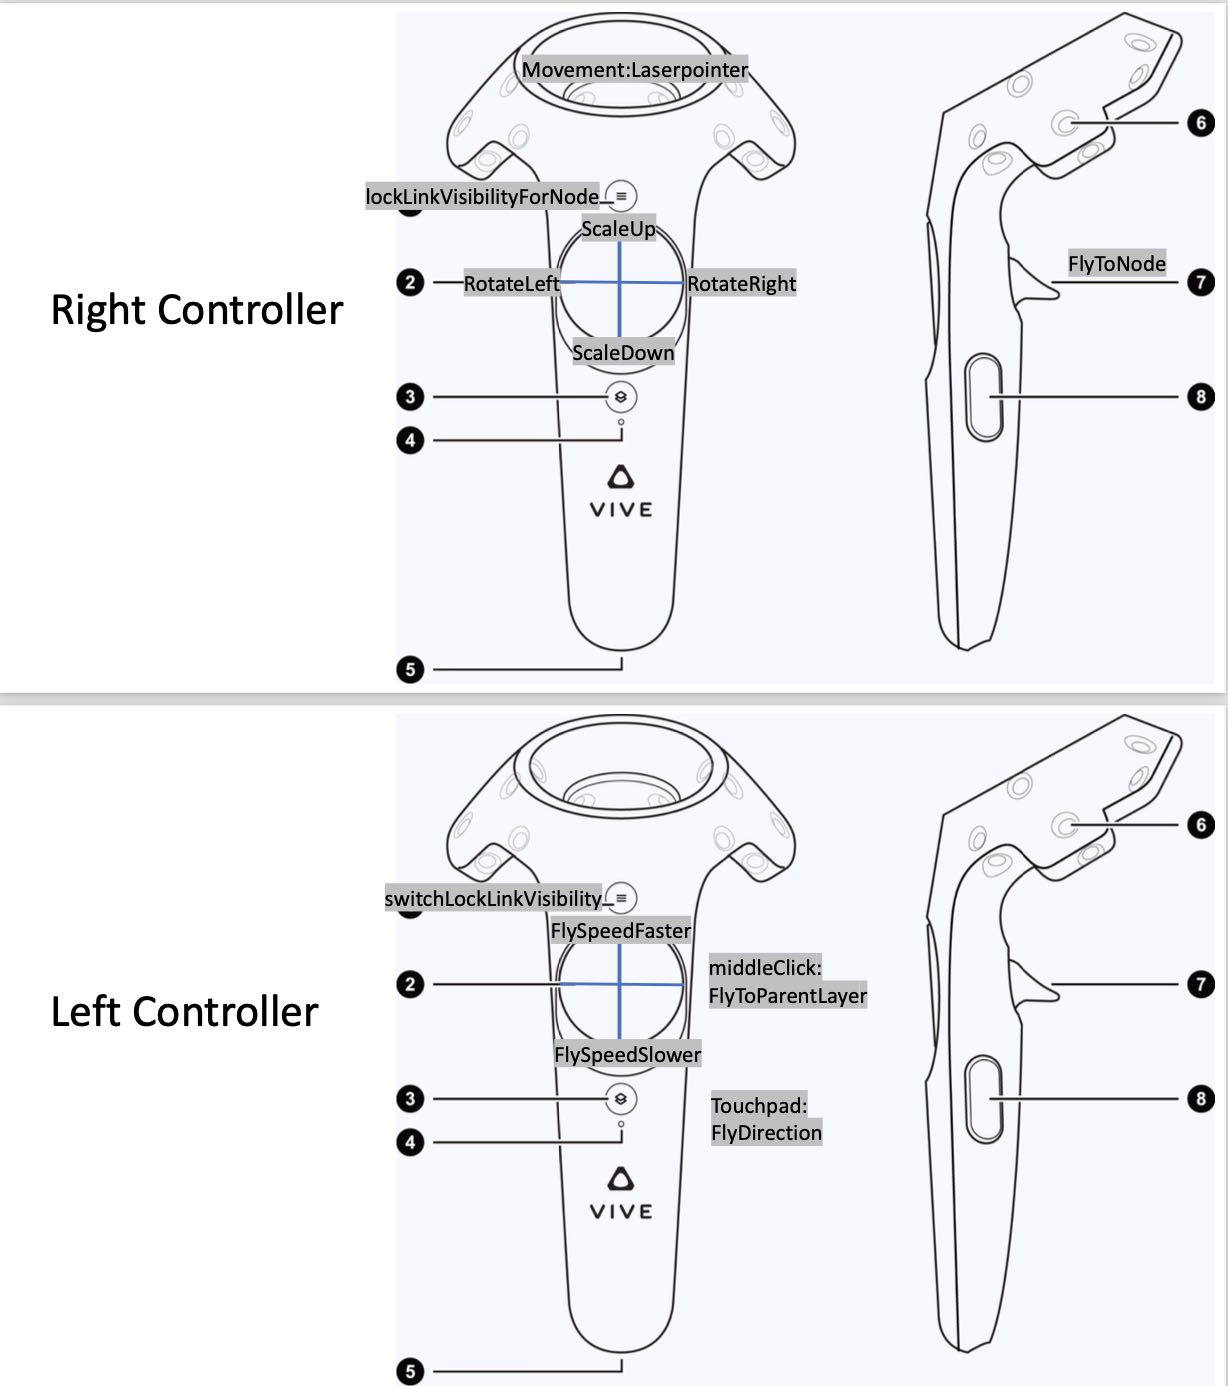
\includegraphics[width=0.5\textwidth]{chapters/graphics/controllerMapping.jpg}
